% !TEX root =../main.tex
\chapter{Estimador de estados}\label{chp:est}

\lettrine[lraise=-0.1, lines=2, loversize=0.2]{E}{n} este capítulo se analizará uno de los elementos que se utilizarán en el siguiente, que es el estimador de estados. En concreto se analiza el que incorpora el autopiloto de código abierto PX4, ya que será este el que se utilizará para la implementación. Previamente, en \cite{arias2019control} se hizo una explicación parcial de este, pero se dejaron atrás algunos detalles como el manejo de las medidas retrasadas. Aquí se explicará esto y además se realizará una simulación que demuestre la eficacia del algoritmo.

\section{Manejo de medidas retrasadas}
En muchas ocasiones se tienen sensores con unos retrasos muy diferentes entre ellos, por ejemplo una IMU es mucho más rápida que el procesamiento de la imagen de una cámara o el GNSS. PX4 lo soluciona añadiendo más elementos a la estructura original de un estimador de estados. Uno de sus elementos es un \textit{Filtro de Kalman Extendido} (EKF). Este no usa las medidas más nuevas que le llegan, si no que las almacena y utiliza las que llegaron hace un determinado tiempo. Corriendo en paralelo, existe un estimador llamado \textit{Filtro de Salida}, el cual sí que utiliza la última medida del acelerómetro y del giróscopo. 

% TODO: Plantear los sensors y que da igual su periodos
% TODO: decir que el periodo de muestreo es de 5 ms

Supongamos que se tiene un sistema que se mueve en el espacio y del que se quiere conocer sus estados, en concreto, su posición, su velocidad y su orientación. Para este objetivo el sistema está dotado de numerosos sensores como son un acelerómetro, un giróscopo, un barómetro, un GNSS o un sensor de flujo óptico. Cada uno de ellos tiene diferentes propiedades en cuanto a retraso, ruido, precisión, etc. Por ejemplo, la medida aportada por el GNSS es la única fuente de posición absoluta, sin embargo, tiene un gran retraso y las medidas que genera se refieren a la posición que se tenía hace un tiempo (generalmente decenas de milisegundos). 

Para explicar un método de cómo afrontar  este problema, se va a poner un ejemplo de la ejecución paso a paso del estimador de estados con diferentes sensores.
Supongamos que en el primera ejecución del estimador, se toma la primera medida de la IMU (acelerómetro y giróscopo). El EKF todavía no la utiliza, si no que la guarda en su buffer (figura \ref{fig:est1}). Conforme llegan nuevas medidas, que ocurre cada 5 ms, estas se introducen en la posición de más a la izquierda del buffer y las que ya estaban se van desplazando hacia la derecha, hasta que llegan a la última celda. La medidas de esta celda situada más a la derecha, son las que son usadas por el EKF. Los estados que este genera y las medidas utilizadas para estimarlos se refieren al \textit{horizonte de tiempo retrasado}. Como se muestra en la figura, el buffer tiene una longitud de 7 celdas, por lo tanto las medidas de la IMU que llegan al EKF siempre serán las que se recogieron hace 30 ms.  

\begin{figure}	
	\centering
	\begin{subfigure}[t]{0.9\textwidth}
		\centering
		\hspace*{-2.0cm}
		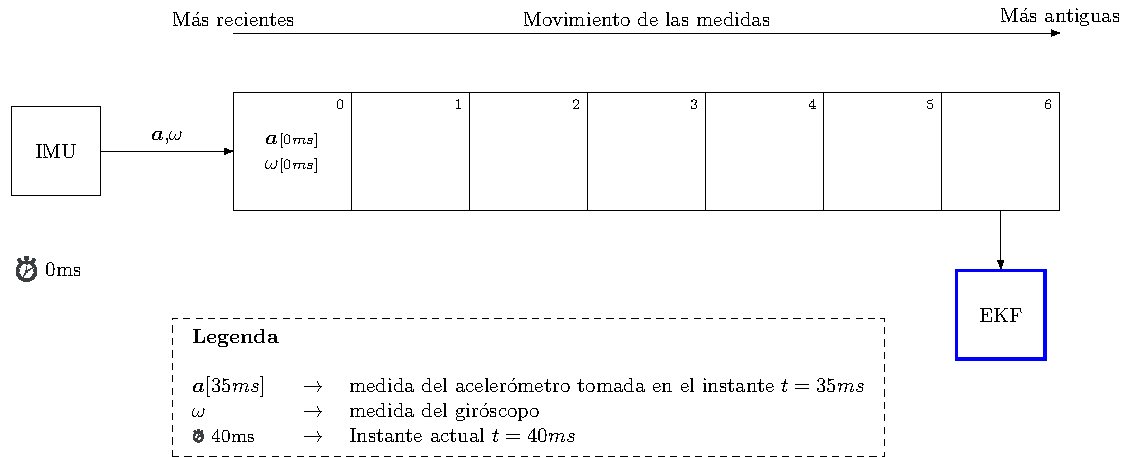
\includegraphics[width=\textwidth]{estimador_px4/tikz/ekf_output_1}
		\caption{Primera medida tomada de la IMU}\label{fig:est1}		
	\end{subfigure}
	\quad
	\begin{subfigure}[t]{1.05\textwidth}
		\centering
		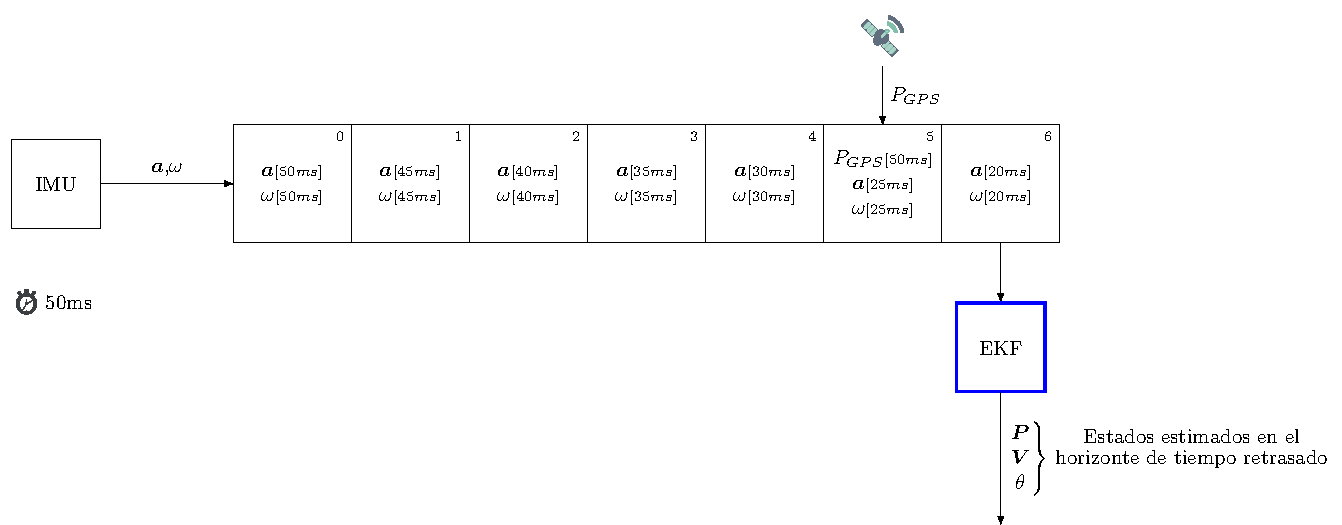
\includegraphics[width=\textwidth]{estimador_px4/tikz/ekf_output_2}
		\caption{Llegada de la medida del GPS}\label{fig:est2}		
	\end{subfigure}
	\begin{subfigure}[t]{0.9\textwidth}
		\centering
		\vspace{1cm}
		\hspace*{-2cm}
		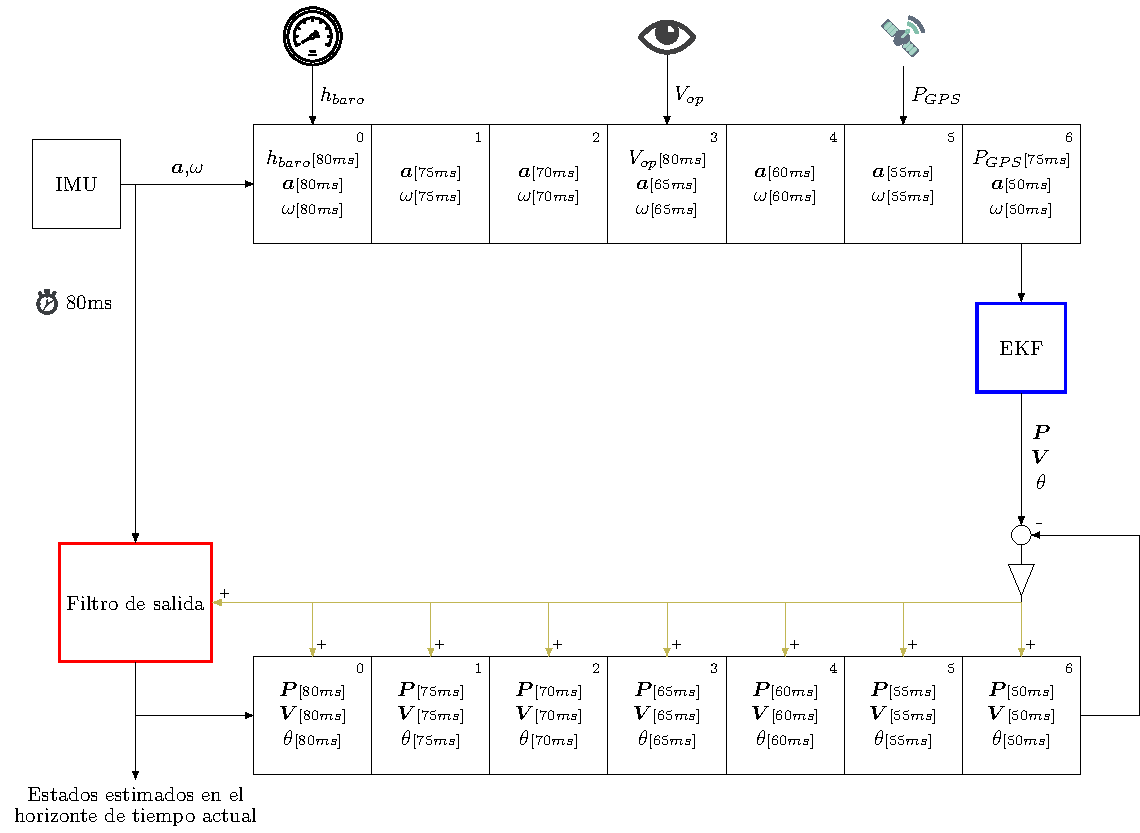
\includegraphics[width=\textwidth]{estimador_px4/tikz/ekf_output_3}
		\caption{Estimador completo}\label{fig:est3}		
	\end{subfigure}
	\quad
	\caption{Manejo de medidas retrasadas}\label{fig:retraso}
\end{figure}

Pasan algunos ciclos más hasta que en el instante 60ms llega la primera medida del GPS, pero esta no se coloca en el extremo izquierdo del buffer junto con las medidas más recientes de la IMU, si no que se lleva directamente a la celda número 5 (ver figura \ref{fig:est2}). En esta también se encuentran las medidas de la IMU tomadas en el instante 35ms, es decir las que fueron tomadas hace 25 ms, que coincide con el retraso que tiene la posición del GPS con respecto a la IMU o lo que es lo mismo, la medida del GPS, corresponde a la posición que tenía el vehículo hace 25 ms. De esta manera se agrupan las medidas que se refieren al mismo instante físico, es decir, el instante en el que llegaron pero {\bfseries compensándose su retraso}. 


De forma paralela se ejecuta el \textit{filtro de salida}, que es otro estimador de estados y para esta explicación se va a suponer que su funcionamiento interno es exactamente igual al del EKF, la única diferencia es que solamente utiliza las medidas de la IMU, en este caso las que se generan más recientemente. Estos estados se refieren al \textit{horizonte de tiempo actual} y son los únicos que se usan para las otras tareas que tenga vehículo, como por ejemplo para alimentar al controlador de orientación, por esta razón se le denomina filtro de salida. El problema que tiene este es que desaprovecha todos los demás sensores que tiene el vehículo, por lo que se le aplica un \textbf{mecanismo de corrección}.  

Este mecanismo está compuesto otro buffer llamado \textit{buffer de salida}, que se comporta de la misma manera que el primero, pero en lugar de guardar medidas, almacena los estados del filtro de salida. Estos estados se van desplazando hacia la derecha hasta que llegan a la última posición del buffer. En esta posición están los estados que se estimaron por el filtro de salida hace 30 ms, que coincide con el retraso que tienen las medidas del la IMU que entran al EKF. Si al EKF solo se le hubiese suministrado las medidas de la IMU, al igual que al filtro de salida, los estados del EKF y los que hay almacenado en esta última celda del buffer de salida coincidirían. Sin embargo, lo que está ocurriendo es que el EKF recoge medidas de otros sensores y por lo tanto no coincidirán. Para realizar la corrección, se calcula la diferencia entre ellos. Esta diferencia se atenúa y se le suma a todos los elementos del buffer de salida, además de al propio filtro de salida. 

En la figura \ref{fig:est3} se ha ilustrado este mecanismo de corrección además de incluir más medidas: la velocidad proporcionada por flujo óptico ($V_{op}$), la cual tiene un retraso de 15ms, y la altura que proporciona el barómetro, que se ha supuesto que no tiene ningún retraso. 

% TODO: comentar otras medidas que han llegado




\subsection{Detalles de implementación}
% tamaño de los buffer
En este apartado se presentan algunos trozos de código de PX4 que implementan lo anteriormente descrito, además de algunos detalles que se han omitido en el apartado anterior para que fuese más fácil su comprensión.

En el apartado anterior se explicó que el error entre los estados estimados en el horizonte de tiempo retrasado y los estados del buffer de salida, se atenuaban (multiplicar por una ganancia menor que 1, mostrado en la figura \ref{fig:est3} como un triángulo) y se le suma a todo el buffer de salida. En el siguiente código se puede ver cómo se ha implementado esto. Se puede ver que la corrección de la velocidad y la posición no solo se calcula a partir del error, sino también a partir de la integral del error, por lo tanto aqui se tiene un control proporcional-integral que tiene como señal de control la corrección al buffer de salida. De esta manera, los estados en el horizonte de tiempo actual, se igualarán a los del horizonte de tiempo retrasado en régimen permanente. 

\begin{codigo}{Correción del buffer de salida. Ubicado en  la línea \href{https://github.com/PX4/PX4-ECL/blob/ec934908900b23ee273d1a9f82364b7b38423200/EKF/ekf.cpp\#L488}{488} del archivo \textit{Firmware/src/lib/ecl/EKF/ekf.cpp}}
\begin{minted}[firstnumber=488]{c++}
void Ekf::applyCorrectionToOutputBuffer(float vel_gain, float pos_gain){
	// calculate velocity and position tracking errors
	const Vector3f vel_err(_state.vel - _output_sample_delayed.vel);
	const Vector3f pos_err(_state.pos - _output_sample_delayed.pos);

	_output_tracking_error(1) = vel_err.norm();
	_output_tracking_error(2) = pos_err.norm();

	// calculate a velocity correction that will be applied to the output state history
	_vel_err_integ += vel_err;
	const Vector3f vel_correction = vel_err * vel_gain + _vel_err_integ * sq(vel_gain) * 0.1f;

	// calculate a position correction that will be applied to the output state history
	_pos_err_integ += pos_err;
	const Vector3f pos_correction = pos_err * pos_gain + _pos_err_integ * sq(pos_gain) * 0.1f;

	// loop through the output filter state history and apply the corrections to the velocity and position states
	for (uint8_t index = 0; index < _output_buffer.get_length(); index++) {
		// a constant velocity correction is applied
		_output_buffer[index].vel += vel_correction;

		// a constant position correction is applied
		_output_buffer[index].pos += pos_correction;
	}

	// update output state to corrected values
	_output_new = _output_buffer.get_newest();
}
\end{minted}
\end{codigo} 

En el código anterior no ha aparecido la corrección de la orientación, y esto es porque requieren que sea tratada a parte. En este estimador, la orientación se expresa en cuaternios y la operación de la corrección no es simplemente una suma como ocurría en el caso de la velocidad, es más complicada y se tardaría demasiado en aplicarla a todos los elementos del buffer. En su lugar, únicamente se aplica una corrección a la orientación estimada en el horizonte de tiempo actual.

\begin{codigo}{Corrección de la orientación. Ubicado en el archivo \textit{Firmware/src/lib/ecl/EKF/ekf.cpp}}
En la línea \href{https://github.com/PX4/PX4-ECL/blob/ec934908900b23ee273d1a9f82364b7b38423200/EKF/ekf.cpp\#L323}{323} se corrige la orientación:
\begin{minted}[firstnumber=323]{c++}
  // Apply corrections to the delta angle required to track the quaternion states at the EKF fusion time horizon
  const Vector3f delta_angle(imu.delta_ang - _state.delta_ang_bias * dt_scale_correction + _delta_angle_corr);
\end{minted}
En la línea \href{https://github.com/PX4/PX4-ECL/blob/ec934908900b23ee273d1a9f82364b7b38423200/EKF/ekf.cpp\#L411}{411} se calcula la ganancia del control
\begin{minted}[firstnumber=411]{c++}
    // calculate a gain that provides tight tracking of the estimator attitude states and
    // adjust for changes in time delay to maintain consistent damping ratio of ~0.7
    const float time_delay = fmaxf((imu.time_us - _imu_sample_delayed.time_us) * 1e-6f, _dt_imu_avg);
    const float att_gain = 0.5f * _dt_imu_avg / time_delay;
    
    // calculate a corrrection to the delta angle
    // that will cause the INS to track the EKF quaternions
    _delta_angle_corr = delta_ang_error * att_gain;
\end{minted}
\end{codigo} 

%La ganancia que multiplica la diferencia entre el filtro de salida y el EKF y que sirve para corregir los estados, se calcula de manera el sistema controlado tenga un factor de amortiguamiento de 0.7.
%\begin{equation}
%K_p=\frac{0.5}{Retraso}
%\end{equation} 
%Puede que este valor se haya sacado de aproximar un retraso e^{sT} por un padé, como viene en https://www.researchgate.net/publication/237396133_RATIONAL_APPROXIMATION_OF_TIME_DELAY
% sin embargo no se como sacar el factor de amortiguamiento de funciones de tranferencia con ceros de fase no mínima.

% TODO: buffer de salida se ejecuta más frecuentemente. 

Tampoco se ha hablado de la longitud de los buffers, la cual hay que determinar antes de empezar a estimar. En el siguiente código se puede ver cómo se calcula la longitud del buffer de medidas de la IMU. Esta se determina de manera que el EKF se ejecutará con un retraso igual al sensor que más retraso tiene.
\begin{codigo}{Cálculo del tamaño del buffer. Ubicado en el archivo \href{https://github.com/PX4/PX4-ECL/blob/ec934908900b23ee273d1a9f82364b7b38423200/EKF/estimator_interface.cpp\#L513}{\textit{Firmware/src/lib/ecl/EKF/estimator\_interface.cpp}}}
\begin{minted}[firstnumber=512]{c++}
  // find the maximum time delay the buffers are required to handle
  const uint16_t max_time_delay_ms = math::max(_params.mag_delay_ms,
  				     math::max(_params.range_delay_ms,
  				       math::max(_params.gps_delay_ms,
  					 math::max(_params.flow_delay_ms,
  					   math::max(_params.ev_delay_ms,
  					     math::max(_params.auxvel_delay_ms,
  					       math::max(_params.min_delay_ms,
  						 math::max(_params.airspeed_delay_ms,
  						       _params.baro_delay_ms))))))));
  
  // calculate the IMU buffer length required to accomodate the maximum delay with some allowance for jitter
  _imu_buffer_length = (max_time_delay_ms / FILTER_UPDATE_PERIOD_MS) + 1;
\end{minted}
\end{codigo} 


\section{EKF para modelo bidimensional}
El objetivo de esta sección, es el de realizar los cálculos necesarios para montar la simulación que vendrá más adelante. Dicha simulación tiene el fin de probar el manejo de medidas retrasadas explicadas anteriormente, no se buscará que sea especialmente realista, añadiendo todos los sensores que se utilizan en la práctica, sino que sea lo más simple posible para centrar la atención en el aspecto que se quiere explicar. Dicho esto, un quadrotor moviéndose en el plano, cuyos únicos sensores son el acelerómetro, giróscopo y GNSS servirá para probar el estimador de estados. 

Para realizar el filtro se tomará prestada la idea de PX4 de suponer que no se tiene conocimiento de ningún aspecto dinámico del vehículo: pares, fuerzas, masa e inercias. En su lugar, se propone un \textbf{modelo cinemático} para la fase de predicción del filtro, en el que las entradas son la aceleración lineal y la velocidad angular que aportan el acelerómetro y giróscopo respectivamente.

Ya que se utilizará un filtro de Kalman discreto, se necesita un modelo discreto en el espacio de estados:
\begin{align}
\bm{X}_{k+1}=
\begin{bmatrix} 
x \\ y \\ V_x \\ V_y \\ \theta
\end{bmatrix}_{k+1}
=& f(\bm{X}_k,\bm{u}_k) + \bm{w}_k \\
\bm{z}_k=
\begin{bmatrix} 
P^{\scalebox{0.5}{GNSS}}_x \\ P^{\scalebox{0.5}{GNSS}}_y
\end{bmatrix}_{k}
 =& h(\bm{X}_k) + \bm{v}_k
\end{align}
Siendo $\bm{X}_{k}$ los estados estimados en la iteración anterior, que están compuestos por la posición, velocidad e inclinación estimadas; $\bm{X}_{k+1}$ los estados predichos, $\bm{u}_k=\begin{bmatrix}a_x & a_y & \omega\end{bmatrix}^T$ el vector de entradas formado por las dos medidas del acelerómetro en los ejes $x$ e $y$ del cuerpo y la medida del giróscopo, $f()$ el modelo de predicción, $\bm{z}_k$ el vector de medidas que en este caso solo contiene la posición del GNSS y $h()$ el modelo de observación. Por último, $\bm{w}_k$ es el ruido de predicción y $\bm{v}_k$ es el de observación, ambos se desarrollarán más adelante.

%Se va a aplicar a un quadrotor en 2 dimensiones, pero el modelo al ser cinemático, se podría aplicar a cualquier otro móvil.

%Estados:
%\begin{align}
%X = 
%\end{align}
Para obtener el modelo de predicción, se realiza la integral discreta a la velocidad,

\begin{align}
\begin{bmatrix} 
x \\ y 
\end{bmatrix}_{k+1}
=
\begin{bmatrix} 
x \\ y 
\end{bmatrix}_k
+
\begin{bmatrix} 
V_x \\ V_y 
\end{bmatrix}_k
\Delta t
\end{align}

también se hace con la velocidad angular,
\begin{align}
\theta_{k+1} = \theta_k + \Delta t \omega
\end{align}

y por último se integra la aceleración en ejes inerciales compensando la medida de la aceleración gravitatoria:
\begin{align}
\begin{bmatrix} 
V_x \\ V_y 
\end{bmatrix}_{k+1}
=
\begin{bmatrix} 
V_x \\ V_y 
\end{bmatrix}_k + 
\Delta t
\begin{bmatrix} 
\cos{\theta} & \sin{\theta} \\ -\sin{\theta} & \cos{\theta}
\end{bmatrix}
\bm{a} +  
\begin{bmatrix} 
0 \\ - g 
\end{bmatrix}\Delta t
\end{align}
Viendo este modelo de predicción $f()$ formado por las tres últimas ecuaciones se puede comprobar que no es lineal con respecto a los estados (debido a las funciones trigonómetricas) y por lo tanto no se puede utilizar un filtro de Kalman convencional, sino uno extendido. Este se basa en realizar una aproximación de primer orden del modelo no lineal:
\begin{align}
\Delta f(\Delta \bm{X}_k) \approx \bm{F}_k\ \Delta \bm{X}_k \end{align} 

Siendo $F_k$ el jacobiano del modelo de predicción con respecto a los estados, que para este caso tiene la siguiente expresión:
\begin{align}
F_k =\left. \frac{\partial f}{\partial X}\right| _{X_{k-1}} =  
\begin{bmatrix} 
%x/X
1 	&0	&\Delta t	&0		&0\\
%y/X
0 	&1	&0		&\Delta t	&0\\
%Vx/X
0 	&0	&1		&0		&\Delta t\left(-a_x\sin{\theta_{k-1}} + a_y\cos{\theta_{k-1}}\right) \\
%Vy/X
0 	&0	&0		&1		&\Delta t\left(-a_x\cos{\theta_{k-1}} - a_y\sin{\theta_{k-1}}\right) \\
%theta/X
0 	&0	&0		&0		&1
\end{bmatrix}
\end{align}




En cuanto al modelo de observación es bastante más sencillo y lineal en este caso, ya que las medidas corresponden directamente con los estados:
\begin{align}
h(\bm{X}_k) =  
\begin{bmatrix} 
x_k \\ y_k
\end{bmatrix}
\end{align}
Lo último que queda por desarrollar del modelo completo son los ruidos, que se suponen que siguen una distribución normal:
\begin{align}
\bm{w}_k \sim \mathcal{N}(0,Q_k) \\
\bm{v}_k \sim \mathcal{N}(0,R_k)
\end{align}
Donde $R_k$ es la matriz de covarianzas del modelo de predicción, que se le ha impuesto el siguiente valor:

\begin{align}
R_k = 
\begin{bmatrix} 
1cm^2 & 0 \\ 0  & 1cm^2\\
\end{bmatrix} 
\end{align}

El ruido del modelo de predicción se calcula en base al ruido de las entradas de la siguiente manera:
%Matriz de covarianzas de la predicción:
\begin{align}
Q_k = 
G_k
\begin{bmatrix} 
\sigma^2_a 	& 0 		& 0\\
0 		& \sigma^2_a 	& 0\\
0 		& 0 		& \sigma^2_\omega\\
\end{bmatrix}
G_k^T
\end{align}
Donde $\sigma_a$ y $\sigma_\omega$ son las desviaciones típicas del acelerómetro y del giróscopo, que se pueden hallar experimentalmente o viendo la hoja de datos de los sensores. $G_k$ es el jacobiano del modelo de predicción con respecto las entradas: 
\begin{align}
G_k =  \frac{\partial f}{\partial \bm{u}_k}=
\begin{bmatrix} 
%x/a,w
0 			&0			&0\\
%y/a,w
0 			&0			&0\\
%Vx/a,w
\Delta t \cos{\theta} 	&\Delta t \sin{\theta}	&0\\
%Vy/a,w
-\Delta t \sin{\theta} 	&\Delta t \cos{\theta}	&0\\
%theta/a,w
0 			&0			&\Delta t		
\end{bmatrix}
\end{align}

Una vez descrito el modelo completo, ya se tiene todo lo que hace falta para ejecutar los pasos del filtro de Kalman extendido. Dichos pasos se implementarán en la simulación siguiente y el lector que quiera saber sobre ellos puede encotrarlos en \cite{arias2019control}.


\section{Simulación del quadrotor y del estimador}
En este apartado se implementará el filtro explicado en este capítulo y pondrá a prueba con un simulador de un quadrotor. Tanto el estimador como el simulador estarán programados en lenguaje Python\footnote{En el apéndice \ref{chp:simu} se encuentra el script \textit{main.py} que implementa toda la simulación de manera independiente, sin necesidad de programas externos}. El simulador será muy sencillo, describirá el movimiento de un quadrotor en el plano al que únicamente se le aplican la fuerza de la gravedad, un empuje y un par. Estos dos últimos serán generados por un controlador de velocidad vertical y un controlador de ángulo, los cuales toman la velocidad, y la inclinación real del vehículo en lugar de medidas ruidosas. Sus referencias se han escogido para que desde el reposo, ascienda unos metros, y luego se desplace hacia la dirección negativa del eje x. 


\begin{figure}
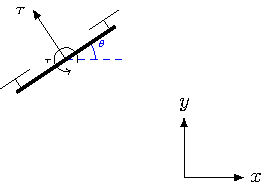
\includegraphics[width=0.5\textwidth]{estimador_px4/tikz/quadrotor_2d}
\caption{Quadrotor en dos dimensiones}
\label{fig:model}
\end{figure}

%Para simular el quadrotor se realiza una integración discreta de :
Para obtener la evolución de la inclinación $\theta$, se utiliza la segunda ley de Newton en el movimiento de rotación, a partir del par de actuación $\tau$ y la inercia $I$:
\begin{align}
        \ddot{\theta} &= \frac{\tau}{I} 
\end{align}

Se obtiene la velocidad angular a partir de la integración descreta de la acelaración,
\begin{align}
        \dot{\theta} &= \dot{\theta}_{i-1} + \Delta t \ddot{\theta} 
\end{align}

y la inclinación a partir de la integral discreta de la velocidad angular:
\begin{align}
        \theta &= \theta_{i-1} + \Delta t \dot{\theta}
\end{align}

En cuanto a la translación, también se aplica la segunda ley de Newton en ejes inerciales:
\begin{align}
         \bm{a}& = \frac{\bm{T_{rot}}+\bm{F_g}}{m}
\end{align}

Donde $\bm{F}_g$ es la fuerza gravitatoria, y $\bm{T}_{rot}$ es el empuje del quadrotor en ejes inerciales que se calcula estableciendo que este siempre tiene la dirección del eje $z$ en ejes cuerpo y magnitud $T$:
\begin{align}
        R &= 
\begin{bmatrix}
\cos{\theta}& -\sin{\theta}\\
\sin{\theta} & \cos{\theta}
\end{bmatrix}\\
         \bm{T_{rot}}&= R  \begin{bmatrix}0\\ T \end{bmatrix}\\
         \bm{F_g}&= \begin{bmatrix}0\\ -m g \end{bmatrix}
\end{align}

La velocidad lineal se obtiene a partir de la aceleración calculada previamente, 

\begin{align}
         \bm{v}& = \bm{v}_{i-1} + \bm{a}\Delta t  
\end{align}

e integrando esta última se obtiene la posición:
 
\begin{align}
        \bm{p} &= \bm{p}_{i-1} + \bm{v}\Delta t  
\end{align}




Una vez se ha simulado esta trayectoria, se pasa ejecutar el estimador de estados. Este toma unas medidas a las que se le ha aplicado un ruido gaussiano y genera su estimación de los estados. Finalmente estos se comparan con los estados reales y se verifica el desempeño del estimador. 

\subsection{Resultados}

El primer experimento que se va a mostrar, al estimador de estados no le va a entrar ninguna otra medida que no sea la del giróscopo y la del acelerómetro. En la figura \ref{fig:simu1} se puede apreciar que la estimación de la posición tiene una deriva, ya que no hay ningún sensor que aporte posición absoluta. 

%\begin{figure}[b]
%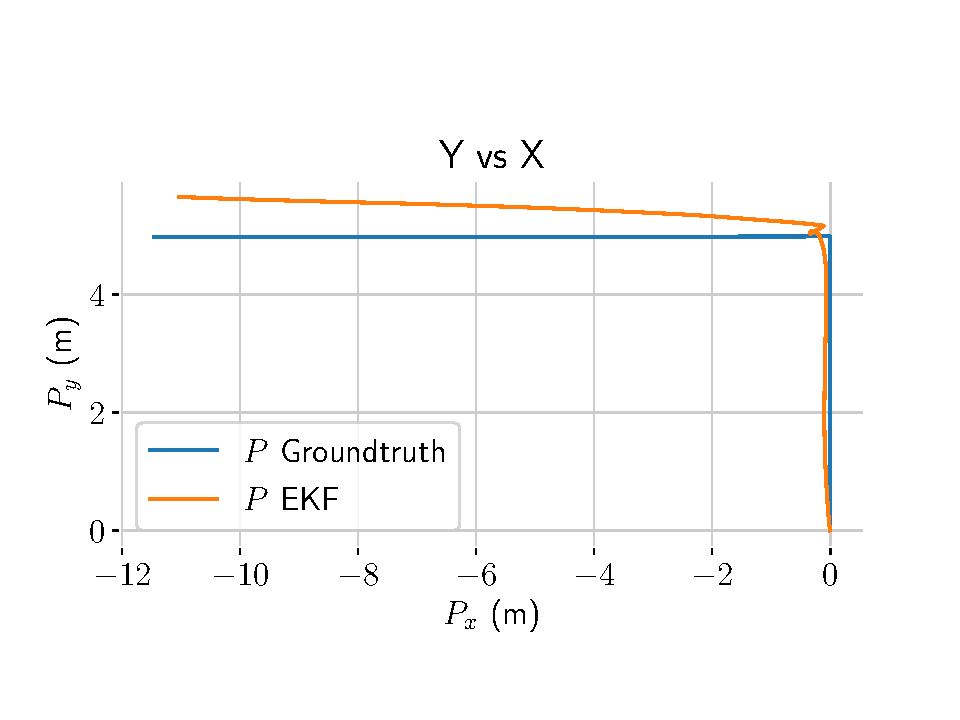
\includegraphics[width=0.5\textwidth]{estimador_px4/im_simu/n_update/tray}

\begin{figure}[b]	
	\centering
	%\hspace*{-0.5cm}
	%\begin{subfigure}[t]{0.49\textwidth}
		\centering
		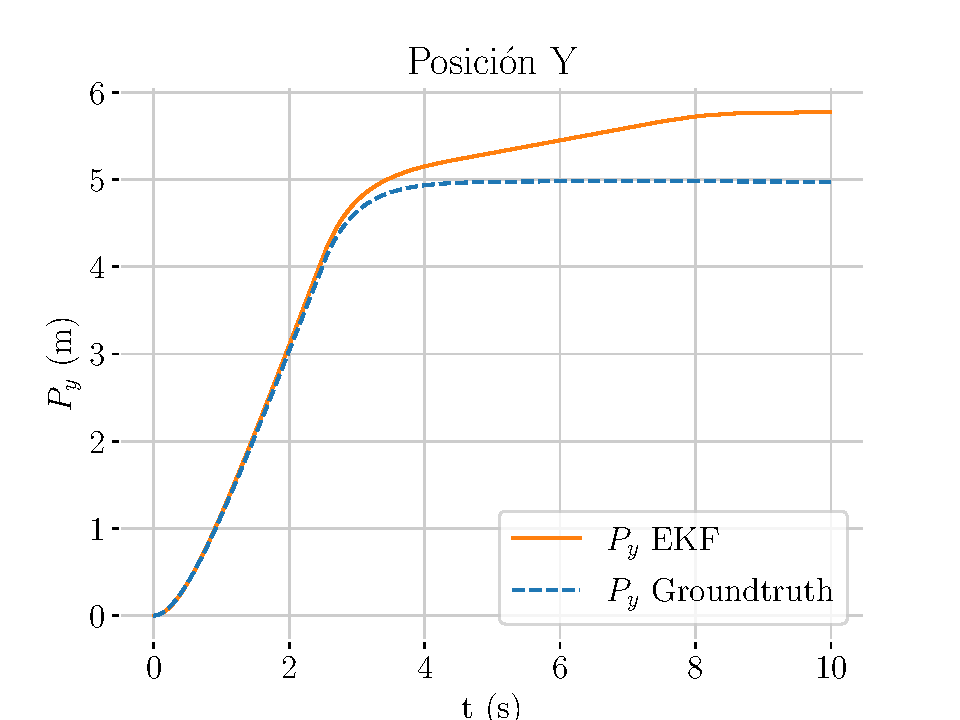
\includegraphics[width=0.5\textwidth]{estimador_px4/im_simu/n_update/y_t}
		%\caption{}
	%\end{subfigure}
	\quad
	\caption{EKF no ejecuta la fase de actualización}
	\label{fig:simu1}
\end{figure}


En el siguiente experimento se va a fusionar un GPS con un retraso de 1 segundo y un periodo de 300ms. Estos valores son poco realistas pero de esta manera se aprecia más la degradación de la estimación. Se puede ver en la figura \ref{fig:no-handle} que el GPS empeora la estimación, ya que en el instante $t=1s$, la estimación se aleja de su valor real porque llega su primera medida. Aquí se puede aprovechar para ver cómo se comporta el filtro de Kalman cuando la medida tiene mucho más error del que se ha especificado. En este caso se impuso que tuviese una desviación típica de 1 centímetro, mientras que en realidad está cometiendo errores de más de un metro a causa del retraso. También se puede ver la dependencia mutua entre todos los estados: la medida del GPS no afecta solo a los estados de la posición, sino que también a la velocidad y a la orientación.  

\begin{figure}[b]	
	\centering
	\hspace*{-0.5cm}
	\begin{subfigure}[t]{0.49\textwidth}
		\centering
		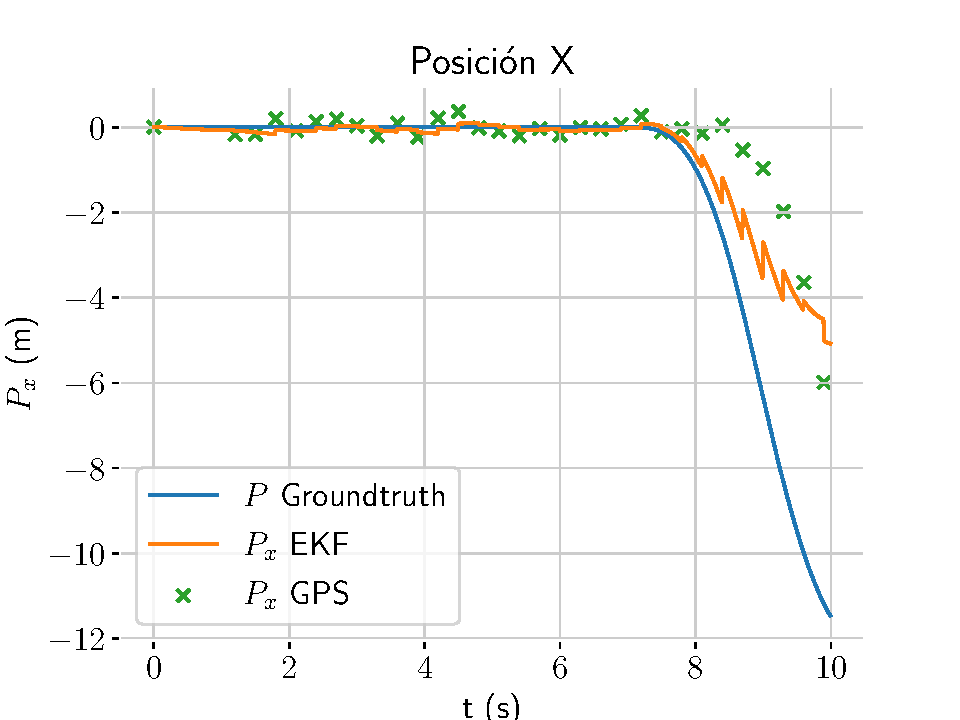
\includegraphics[width=\textwidth]{estimador_px4/im_simu/no_handle_delay/x_t}
		\caption{}
	\end{subfigure}
	\quad
	\begin{subfigure}[t]{0.49\textwidth}
		\centering
		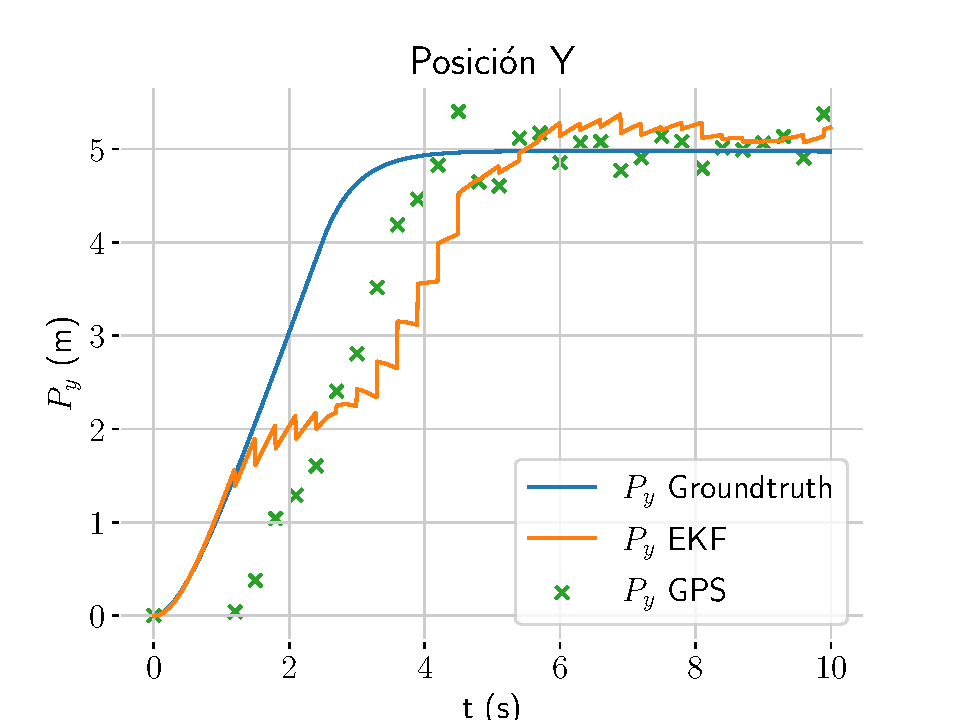
\includegraphics[width=\textwidth]{estimador_px4/im_simu/no_handle_delay/y_t}
		\caption{}
	\end{subfigure}
	\quad
	\hspace*{-0.5cm}
	\begin{subfigure}[t]{0.49\textwidth}
		\centering
		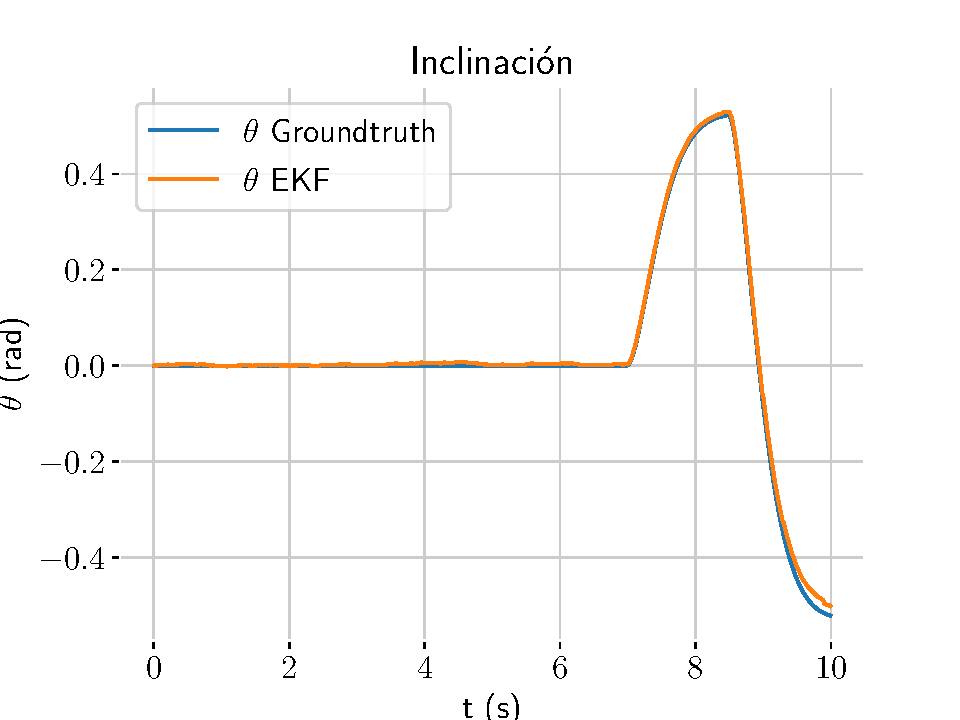
\includegraphics[width=\textwidth]{estimador_px4/im_simu/no_handle_delay/theta}
		\caption{}
	\end{subfigure}
	\quad
	\begin{subfigure}[t]{0.49\textwidth}
		\centering
		\includegraphics[width=\textwidth]{estimador_px4/im_simu/no_handle_delay/vx}
		\caption{}
	\end{subfigure}
	\quad
	\caption{Fusión del GPS con retraso}
	\label{fig:no-handle}
\end{figure}

En el tercer experimento se ha realizado el manejo de los retrasos explicado en este capítulo. En la figura \ref{fig:handle} se tiene que, aunque la medida esté retrasada un segundo, esta no se ve degradada por el GPS ya que se le está compensando su retraso antes de fusionarlo con las medidas de la IMU. Es más, la estimación es mejor que en los dos casos anteriores. En la imagen \ref{fig:py-error} se puede ver la desviación típica que estima el filtro, que tiene forma de diente de sierra debido a la llegada periódica de las medidas del GPS, comparado con los errores reales: el del filtro de salida y el del EKF, que se calcula como la diferencia con el groundtruth retrasado la misma cantidad de tiempo que el filtro de Kalman extendido. En este último caso, el error estimado no se aleja mucho del real, pero en el caso del filtro de salida este error es mayor. 

\begin{figure}	
	\centering
	\hspace*{-0.5cm}
	\begin{subfigure}[t]{0.49\textwidth}
		\centering
		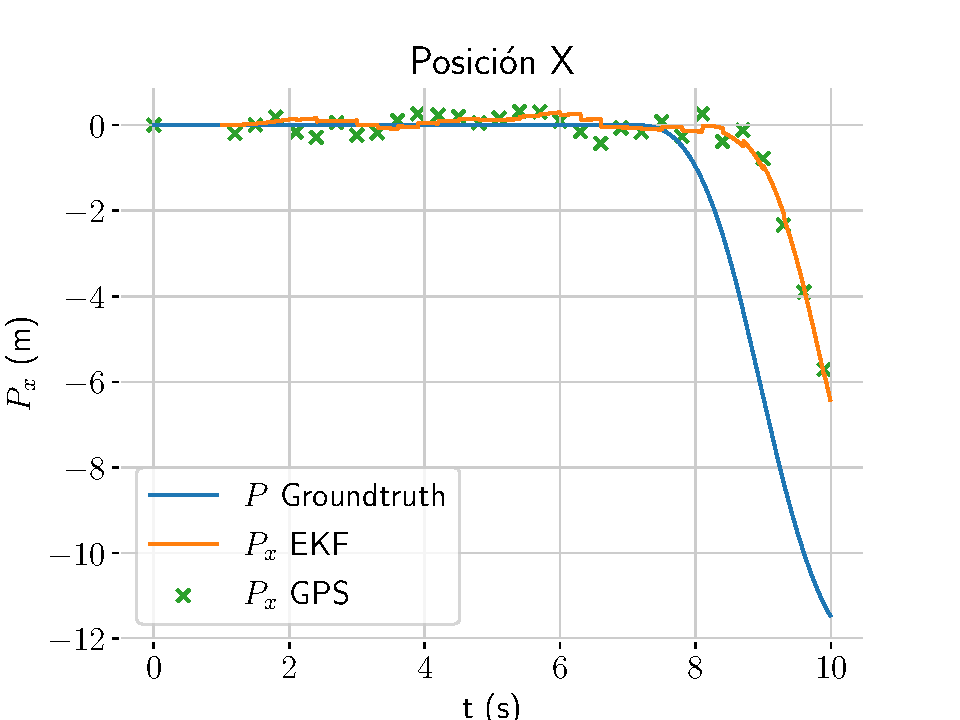
\includegraphics[width=\textwidth]{estimador_px4/im_simu/handle_delay/x_t}
		\caption{}
	\end{subfigure}
	\quad
	\begin{subfigure}[t]{0.49\textwidth}
		\centering
		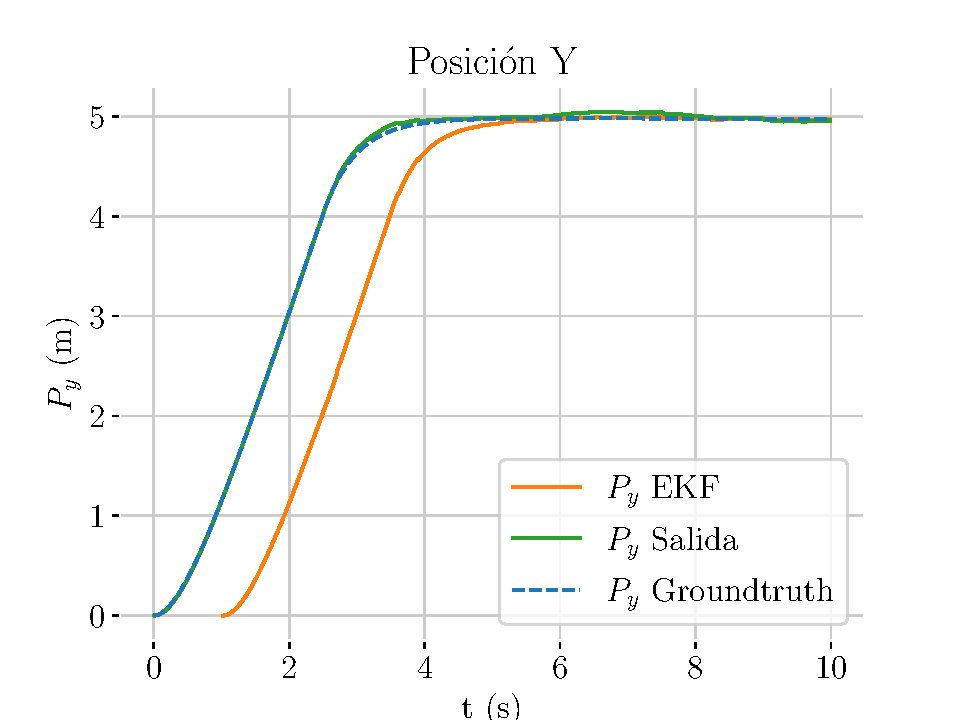
\includegraphics[width=\textwidth]{estimador_px4/im_simu/handle_delay/y_t}
		\caption{}
	\end{subfigure}
	\quad
	\hspace*{-0.5cm}
	\begin{subfigure}[t]{0.49\textwidth}
		\centering
		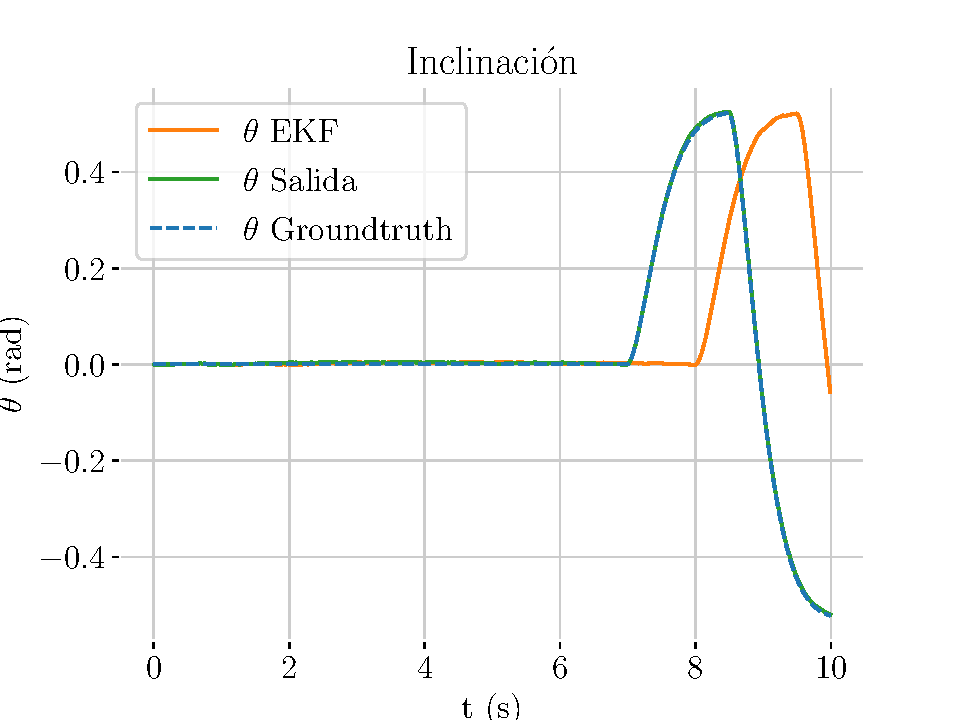
\includegraphics[width=\textwidth]{estimador_px4/im_simu/handle_delay/theta}
		\caption{}
	\end{subfigure}
	\quad
	\begin{subfigure}[t]{0.49\textwidth}
		\centering
		\includegraphics[width=\textwidth]{estimador_px4/im_simu/handle_delay/vx}
		\caption{}
	\end{subfigure}
	\quad
	\hspace*{-0.5cm}
	\begin{subfigure}[t]{0.49\textwidth}
		\centering
		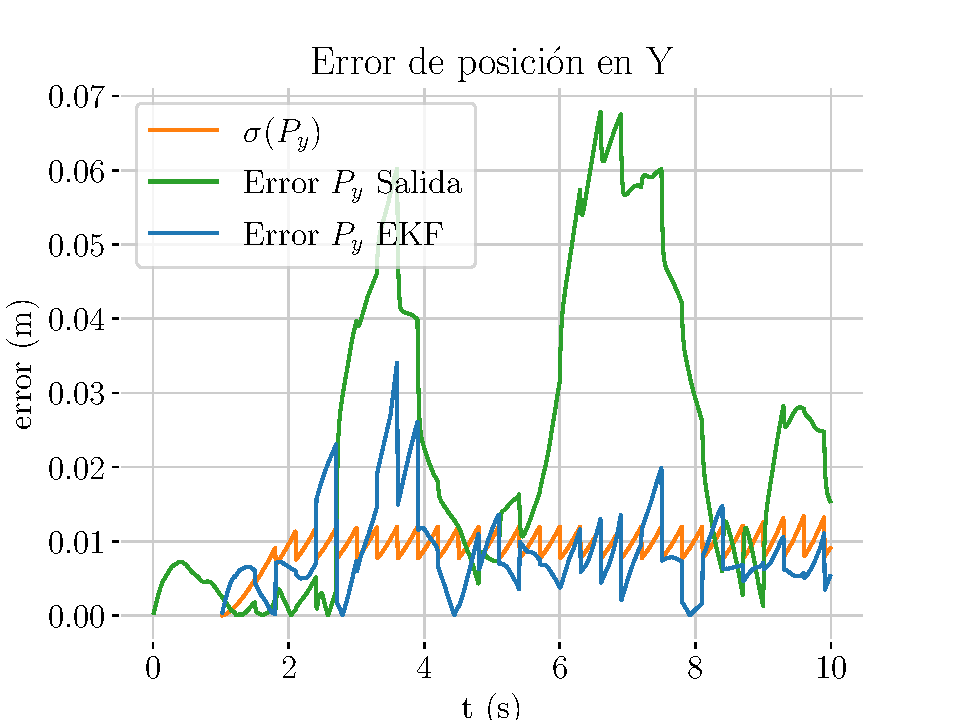
\includegraphics[width=\textwidth]{estimador_px4/im_simu/handle_delay/Py_error}
		\caption{}
		\label{fig:py-error}
	\end{subfigure}
	\quad
	\begin{subfigure}[t]{0.49\textwidth}
		\centering
		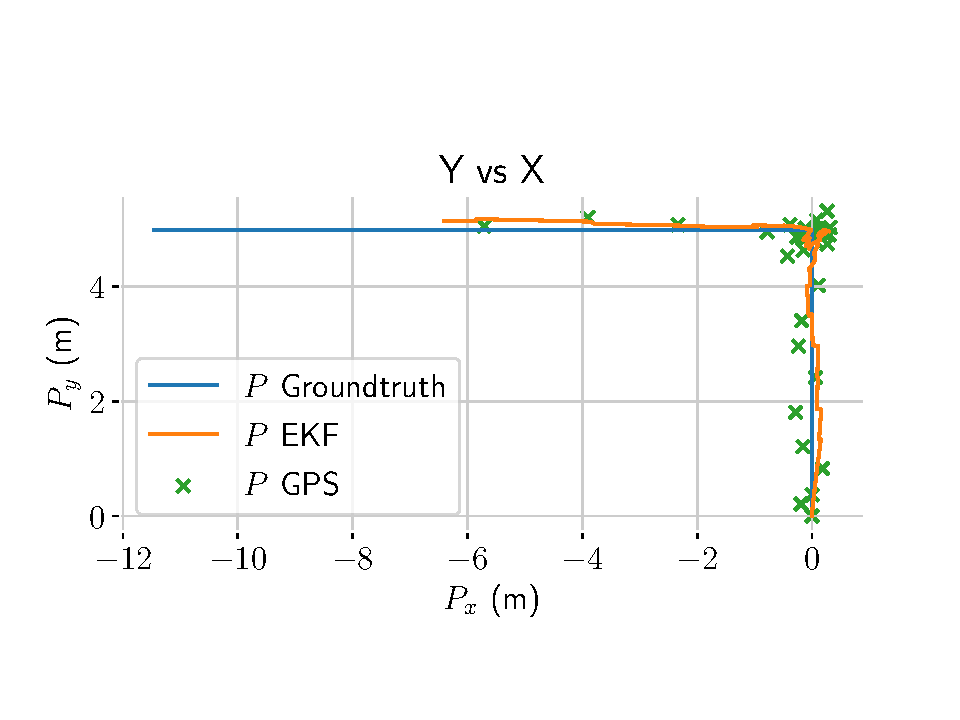
\includegraphics[width=\textwidth]{estimador_px4/im_simu/handle_delay/tray}
		\caption{}
	\end{subfigure}
	\quad
	\caption{Experimento con manejo de medidas retrasadas}
	\label{fig:handle}
\end{figure}





\endinput
